\documentclass[exercice]{thedocument}%
\startdatakeys
\source{}
\cycle{}
\competencesDuSocle{}
\connaissancesRequises{}
\competencesTravaillees{}
\enddatakeys
\begin{document}%
Sur la figure ci-contre, qui n'est pas en vraie grandeur, le point C est le
point d'intersection des droites (BE) et (AD).\vskip10pt
\begin{minipage}[carreau]{.5\linewidth}
    \begin{enumerate}
        \item Démontrer que le triangle ABC est rectangle en C.
        \item Calculer l'aire du triangle ABC.
        \item Calculer une valeur approchée au degré près de l'angle $\widehat{\text{BAC}}$.
        \item Calculer le périmètre du triangle CDE.
        \item Les droites (AB) et (DE) sont-elles parallèles ?
    \end{enumerate}
\end{minipage}\hskip50pt minus 30pt
    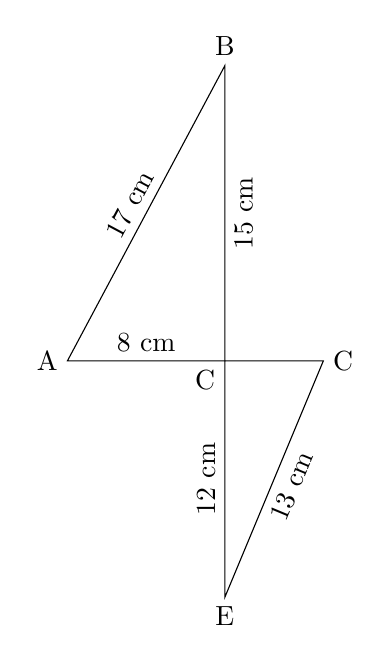
\begin{tikzpicture}[scale=0.25, baseline=(current bounding box.center)]
        \coordinate[label=below left:C](C)at(0,0);
        \coordinate[label=left:A](A)at(-8,0);
        \coordinate[label=right:C](D)at(5,0);
        \coordinate[label=B](B)at(0,15);
        \coordinate[label=below:E](E)at(0,-12);
        \path(A)--(B)node[midway,above,sloped]{17 cm};
        \path(C)--(B)node[midway,below,sloped]{15 cm};
        \path(A)--(C)node[midway,above,sloped]{8 cm};
        \path(E)--(C)node[midway,above,sloped]{12 cm};
        \path(E)--(D)node[midway,below,sloped]{13 cm};
        \draw(A)--(D)--(E)--(B)--cycle;
    \end{tikzpicture}
\end{document}
